\section{Évaluation des extensions proposées}\label{sec:contribs:perf_eval}


Nous avons évalué les différentes améliorations proposées dans les sections~\ref{sec:openmp:langage} et~\ref{sec:openmp:runtime} sur les machines idchire et brunch, décrites en détails dans la section~\ref{sec:contribs:machines}.

La section suivante décrit les différents logiciels que nous avons utilisé pour nos expériences, ainsi que les modifications apportées le cas échéant ; et la section~\ref{sec:contribs:perf_eval:resultats} aborde point par point les extensions proposées.
Enfin la section~\ref{sec:contribs:perf_eval:libkomp} discute de l'application de nos idées dans un support exécutif différent, avec également une évaluation de performances.


\subsection{Logiciels}

Les logiciels utilisés pour nos expériences peuvent être divisé en trois catégories~:
\begin{itemize}
  \item Les applications utilisées
  \item Les supports exécutifs
  \item Les bibliothèques externes
\end{itemize}

Les applications et les supports exécutifs utilisées ont pu subire quelques modifications afin d'incorporer les modifications d'OpenMP proposées.
Ces changements sont décrits ci-dessous.
Nous n'avons effectué aucune modification aux bibliothèques externes, mais il est important de faire un point dessus, étant donné qu'une partie des performances peut en dépendre.

\subsubsection{Applications utilisées}

Les applications utilisées pour ces expériences proviennent des KASTORS\footnote{https://gitlab.inria.fr/openmp/kastors, branche 'affinity'}.

Nous avons ajouté une clause \emph{affinity} dans certaines applications~: dans le cas des applications d'algèbre linéaire, les tâches de calculs dépendent d'un ou plusieurs blocs de données. Nous avons ajouté une affinité entre chaque tâche et les données qu'elle écrit.
Dans le cas des applications de type stencil, nous avons ajouté une affinité vers un cœur précis pour les tâches successives.


\subsubsection{Supports exécutifs}


\paragraph{XKAAPI :} nous avons implémentés les trois types d'extensions proposés dans la section~\ref{sec:openmp:runtime}, à savoir les différentes stratégies de distribution des données, les stratégies de sélection lors du vol de travail, et les stratégies de placement des tâches prêtes.
Ces modifications ont été rassemblées dans une version spécifique de XKAAPI~\footnote{https://scm.gforge.inria.fr/anonscm/git/kaapi/xkaapi.git, branche 'public/europar2016'}.


Nous avons pris comme base de comparaison les supports exécutifs fournis avec les compilateurs existant au moment de nos propositions.

\paragraph{GCC/libGOMP :} nous avons utilisé la version 5.2.0 comme référence, sans y apporter de modification.

\paragraph{Clang/libOMP :} nous avons utilisé la version 3.8. Bien que le support exécutif (libOMP) n'ait pas été modifié, le compilateur (Clang) a subit des modifications afin de supporter les clauses décrites dans la section~\ref{sec:openmp:langage}.

\subsubsection{Bibliothèques externes}

\paragraph{BLAS :} les applications d'algèbre linéaire des KASTORS dépendent de la bibliothèque BLAS.
Pour les expériences effectuées dans la section~\ref{sec:contribs:perf_eval:resultats}, nous avons utilisé la bibliothèque OpenBLAS~2.15 pour fournir les noyaux de calculs de base.


\paragraph{hwloc :} cette bibliothèque fournie les informations sur la hiérarchie de la machine, ainsi que des fonctions d'allocation de mémoire selon différentes politique (voir section~\ref{sec:context:os:lib}). Nous avons utilisé la version 1.11.0.

\paragraph{numactl :} nous avons utilisé \emph{numactl} pour certaines courbes de référence. \emph{numactl} est fourni par libNUMA ; nous avons utilisé la version par défaut fourni par le fabricant de la machine.


\subsection{Résultats}\label{sec:contribs:perf_eval:resultats}

\begin{todo}
  C'est plus une note qu'un TODO : j'ai volontairement ignoré les résultats sur brunch dans cette section.
  L'éval des perfs a été faite avec kaapi, et on avait pas du tout fait tourné ça sur brunch.
  En revanche il y a une section à part pour le nouveau libKOMP, dans lequel on peut montrer l'éval de perf sur brunch et idchire. (et probablement étendre avec une section sur les résultats du simulateur, quand ça sera prêt.
\end{todo}

Les résultats obtenus sont illustrés ci-dessous, dans trois sections abordant des points important~: la distribution des données, la prise en compte de la localité des données lors de l'exécution, et la possibilité de restreindre le vol de travail.

\subsubsection{Impact de la distribution des données}

\begin{figure}[ht]
  \centering
  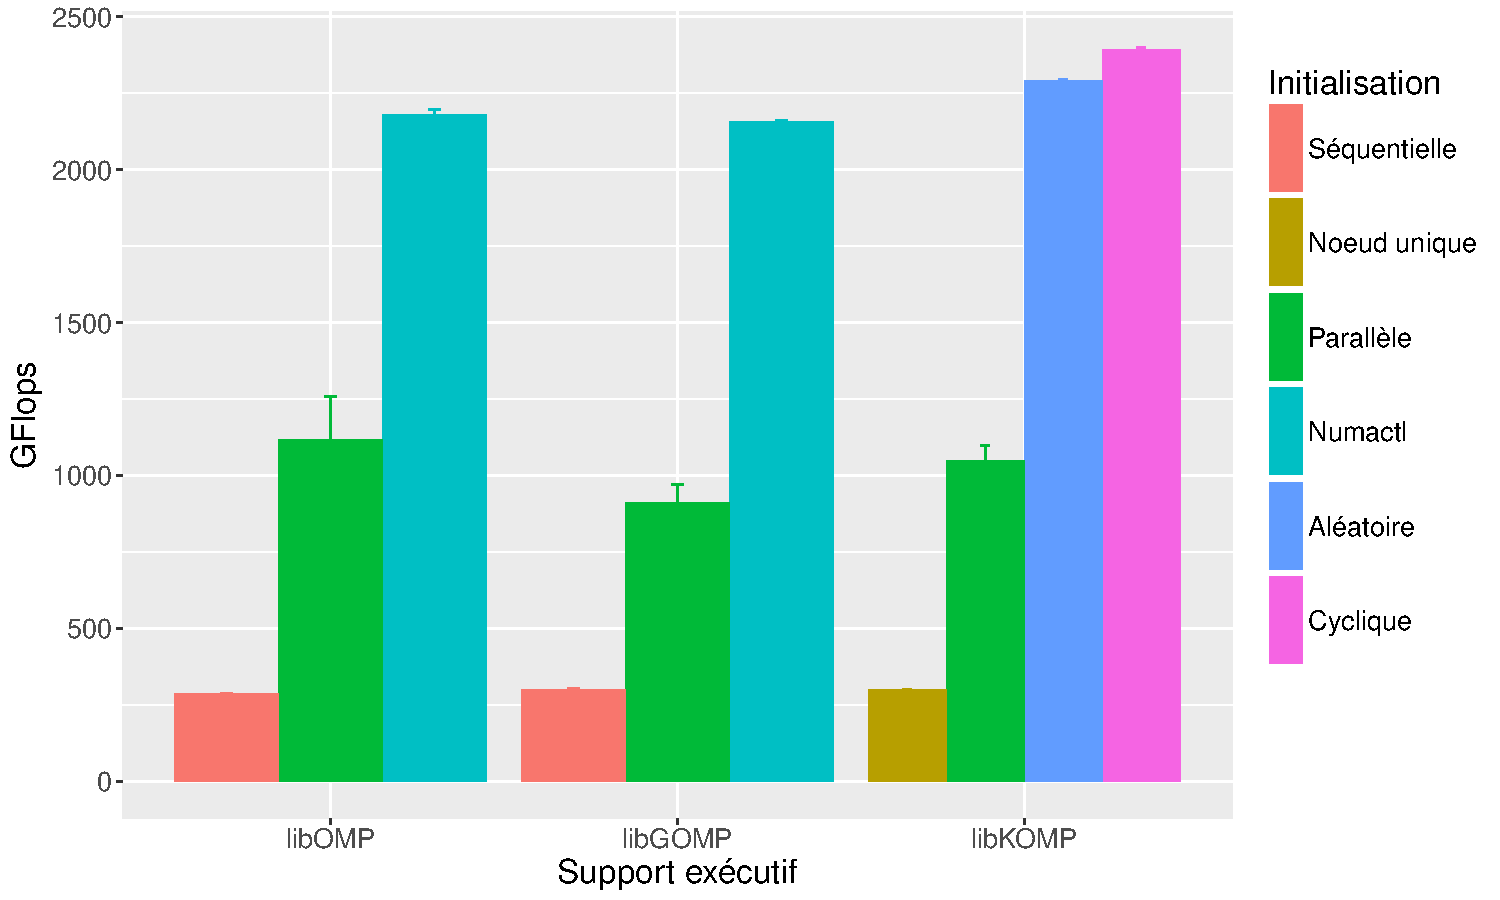
\includegraphics[width=\textwidth]{graph_distrib_data_idchire}
  \caption{Performances des différentes stratégies pour Cholesky en fonction de la distribution de données (N=32768, BS=512)}\label{fig:contribs:perf_eval:distrib-idchire}
\end{figure}

La figure~\ref{fig:contribs:perf_eval:distrib-idchire} montre un exemple représentatif du comportement de la factorisation de Cholesky par bloc, en fonction du type de distribution de données. La taille de matrice utilisée est 32768, et la taille de bloc est 512, et la performance affichée est celle obtenue avec l'ensemble des 192 cœurs d'idchire.
La distribution \emph{Native} correspond à l'exécution du programme original, avec différent types d'initialisation.
Les deux autres distributions, \emph{Cyclique} et \emph{Aléatoire} correspondent aux distributions que nous avons implémentées, et à titre comparatif plusieurs stratégies d'ordonnancement sont données.

La première chose à remarquer est que l'initialisation séquentielle de base - \emph{libGOMP Séquentiel} - propose sans surprise des performances désastreuses. L'utilisation de \emph{numactl} (\emph{libGOMP numactl}) permet d'améliorer les performances mais cela reste largement en dessous de ce qu'on peut obtenir avec une initialisation parallèle.
Toutes les autres stratégies utilisent une initialisation parallèle dans laquelle chaque tâche est responsable de l'initialisation d'un bloc de données.
Ainsi même si \emph{libGOMP Parallèle} n'a pas de contrôle sur le placement de ces tâches d'initialisation (et donc sur le placement des données, comme expliqué dans la section~\ref{sec:openmp:langage:init}), il y a quand même une distribution sur la machine~: il y a 64 blocs à allouer sur 24 nœuds et libGOMP fonctionne par vol de travail, toutes les tâches seront donc effectuées par différents cœurs répartis sur toute la machine.

Parmi nos stratégies, \emph{sRand/pLoc} correspond à une stratégie basique de vol de travail aléatoire, comparable à ce qu'utilise libGOMP.
Ajouter une distribution de données spécifique assure que la distribution des tâches ne repose pas sur l'ordonnancement par défaut du support exécutif, et l'ordre parfois non contrôlé dans lequel les threads viennent voler du travail.
Bien que la différence ne soit que de quelques dizaines de GFlops, la distribution \emph{Cyclique} sur l'ensemble des nœuds NUMA semble être plus avantageuse que la distribution \emph{Aléatoire} sur l'ensemble des stratégies d'ordonnancement testé, et c'est celle qu'on a retenu pour les expériences des sections suivantes.

Le point important à retenir de ces résultats est qu'il est absolument crucial que l'initialisation des données à <<grouper>> ensemble soit faite par une tâche dédiée, afin que même si aucun contrôle n'est effectué il y ait tout de même une distribution naturelle possible des données.



\subsubsection{Étude comparative des stratégies et impact de l'affinité}

La section~\ref{sec:contrib:ws:heuristics} décrit plusieurs stratégie de sélection et de placement des tâches.
Parmi les nombreuses combinaisons possibles nous en avons choisi 7 qui nous semblaient pertinentes.

\begin{figure}[ht]
  \centering
  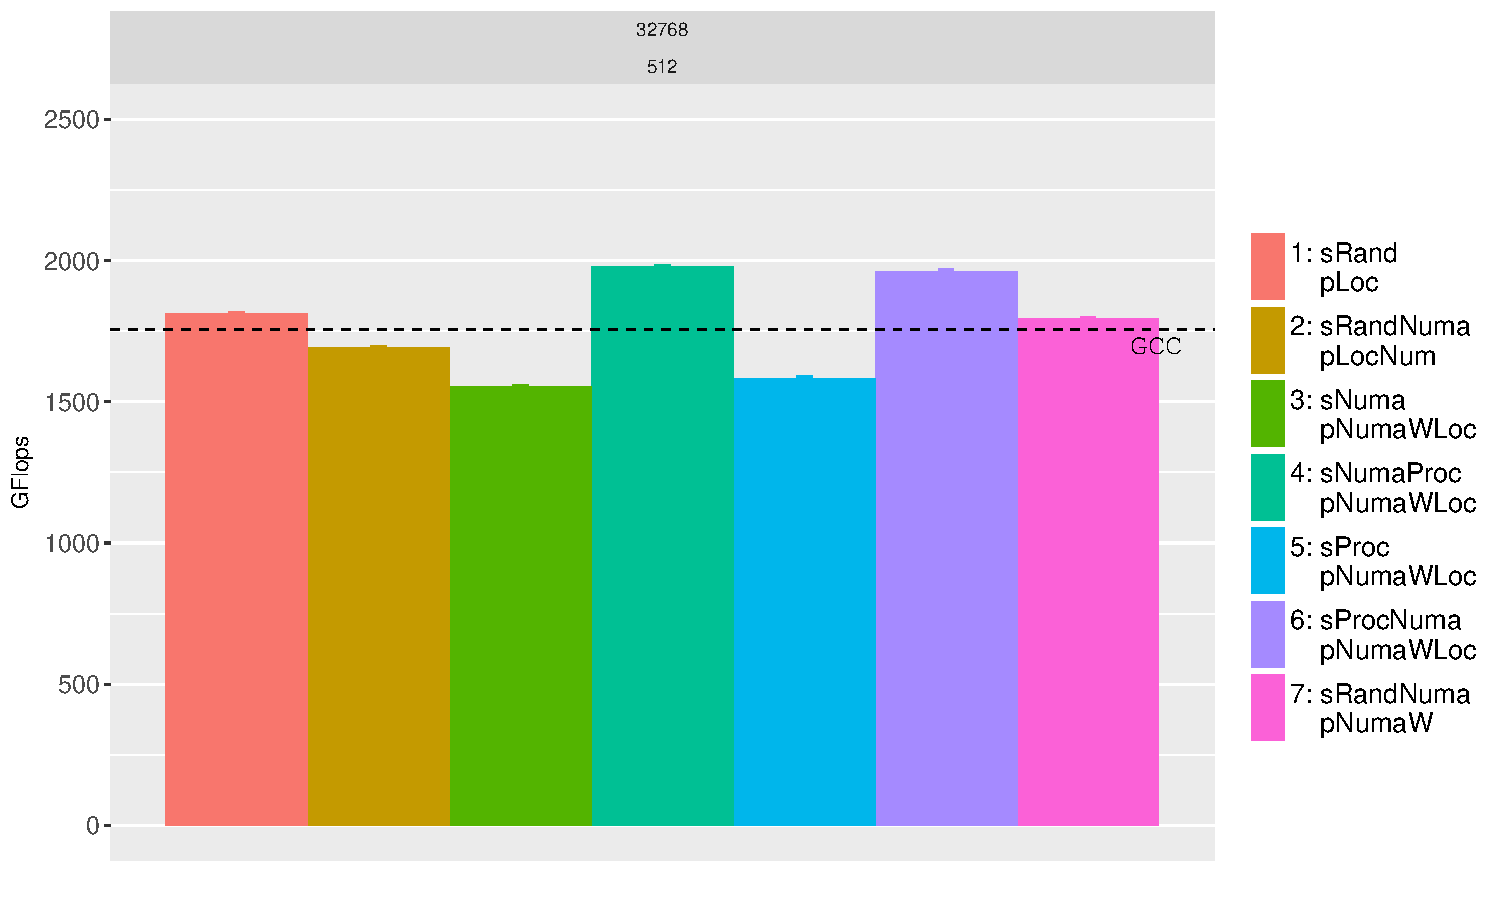
\includegraphics[width=\textwidth]{graph_all_strat_idchire}
  \caption{Performances des différentes stratégies pour Cholesky (N=32768, BS=512)}\label{fig:contribs:perf_eval:eval-strategies}
\end{figure}

La figure~\ref{fig:contribs:perf_eval:eval-strategies} regroupe les performances de ces stratégies sur un exemple représentatif de leur comportement~: une factorisation de Cholesky sur une matrice de taille 32768 avec une taille de bloc de 512.
Les meilleures performances de GCC sont indiquées comme repère.

Parmi les stratégies choisies il y a~:
\begin{itemize}
  \item Deux stratégies <<naïves>> avec vol de travail aléatoire, soit au niveau des cœurs (1), soit au niveau des nœuds (2)
  \item Une stratégie prenant en compte l'affinité, mais n'effectuant la gestion des tâches qu'au niveau des nœuds (7)
  \item Quatre stratégies prenant en compte l'affinité et favorisant un placement des tâches à deux niveaux (dans la file du nœud NUMA si l'affinité pointe sur un nœud distant, ou dans la file du cœur courant si l'affinité pointe vers le nœud local). La différence entre les stratégies 3, 4, 5, et 6 réside dans la stratégie de sélection des victimes lors du vol de travail.
\end{itemize}

La première chose à remarquer est que les stratégies a priori naïves offre des performances tout à fait acceptables (libGOMP via GCC, 1, et 2) !

Deux stratégies sortent clairement du lot~: 4 et 6. Leur spécificité commune est qu'elles utilisent complètement les deux niveaux de hiérarchie, tant lors du placement des tâches que lors de la sélection d'une victime à voler.
Leur différence est uniquement l'ordre de parcours des files de tâches~: 4 commence par essayer de voler les nœuds puis ensuite les cœurs, 6 fait l'inverse (une description détaillée avec des schémas est donnée dans la section~\ref{sec:contrib:ws:heuristics}).

Conserver un placement hiérarchique mais avoir une sélection principalement sur un seul niveau de hiérarchie n'est pas concluant (3 et 5).
Prendre en compte l'affinité mais ne faire du placement ou de la sélection que parmi les files des nœuds NUMA (7) offre des performances juste équivalente à une stratégie basique de vol de travail (1).

Dans ce type de circonstances on peut donc conclure que l'ajout d'une affinité sur les tâches, couplée à une hiérarchisation du support exécutif, permet d'améliorer significativement les performances.


\begin{figure}[h!]
  \centering
  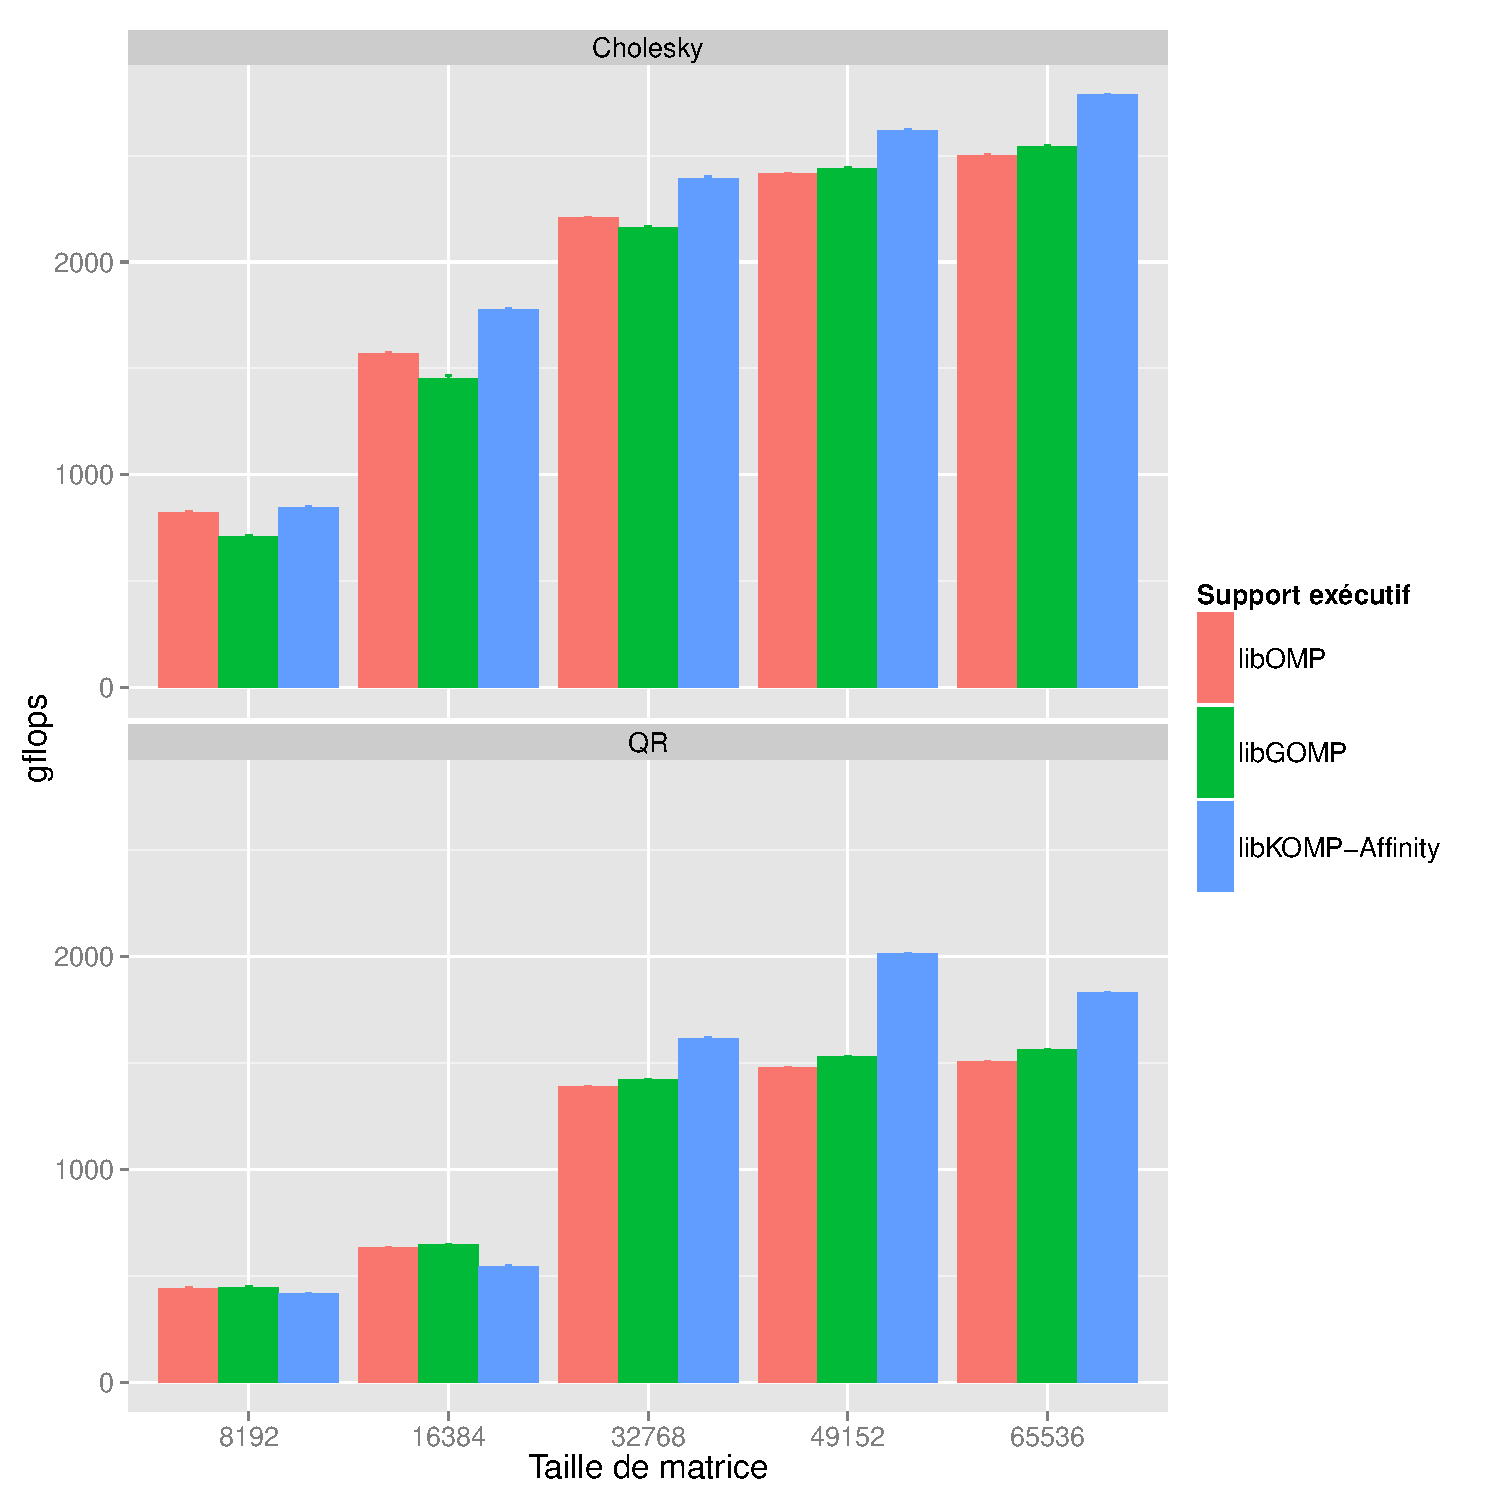
\includegraphics[width=\textwidth]{graph_details_qr_cholesky_idchire}
  \caption{Comparaison de trois stratégies sur QR et Cholesky, en fonction de la taille de matrice}\label{fig:contribs:perf_eval:eval-qr-cholesky}
\end{figure}

Nous avons bien évidemment effectué d'autres expériences sur des applications et tailles différentes pour regarder si cette tendance se confirmait. Nous avons choisi trois stratégies (1, 4, 7) parmi celles présentées dans la figure~\ref{fig:contribs:perf_eval:eval-strategies}, que nous avons évaluées sur les factorisations QR et Cholesky, avec des tailles de matrice variant entre 16384 et 65536, en utilisant la meilleure taille de bloc que nous avons pu trouver pour chaque taille de matrice.

La figure~\ref{fig:contribs:perf_eval:eval-qr-cholesky} montre les résultats obtenus.
Pour la taille de matrice 16384 la taille de bloc est de 256, pour les autres elle de 512.
On a donc une différence claire vis à vis du cache L3~: dans le cas des blocs de taille 256 l'ensemble des données de calcul pour chaque noyau de l'application tient dans le cache L3, ce qui n'est pas le cas pour les blocs de taille 512.
Compte tenu des résultats montrés dans la section~\ref{sec:contribs:apps:cholesky:locality}, il est donc logique d'observer l'amélioration significative des performances pour de grande tailles de blocs (nécessaires pour les grandes tailles de matrices), et une différence relativement faible concernant les tailles de blocs plus petites.


\subsubsection{Affinité stricte}

La section~\ref{sec:openmp:langage:affinity} introduit la clause affinité en précisant que l'utilisateur peut spécifier une affinité \emph{stricte}, restreignant ainsi les décisions d'ordonnancement du support exécutif.
Cette fonctionnalité n'a pas été utilisée pour les applications d'algèbre linéaire, car dans les cas que nous avons étudiés il était plus rentable de payer le coût de transfert des blocs de données plutôt que de se priver du parallélisme disponible.
Ce n'est évidemment pas le cas pour toutes les applications, et les applications stencil, comme Jacobi, peuvent grandement bénéficier d'une restriction d'affinité aux ressources proches.

\begin{figure}[ht]
  \centering
  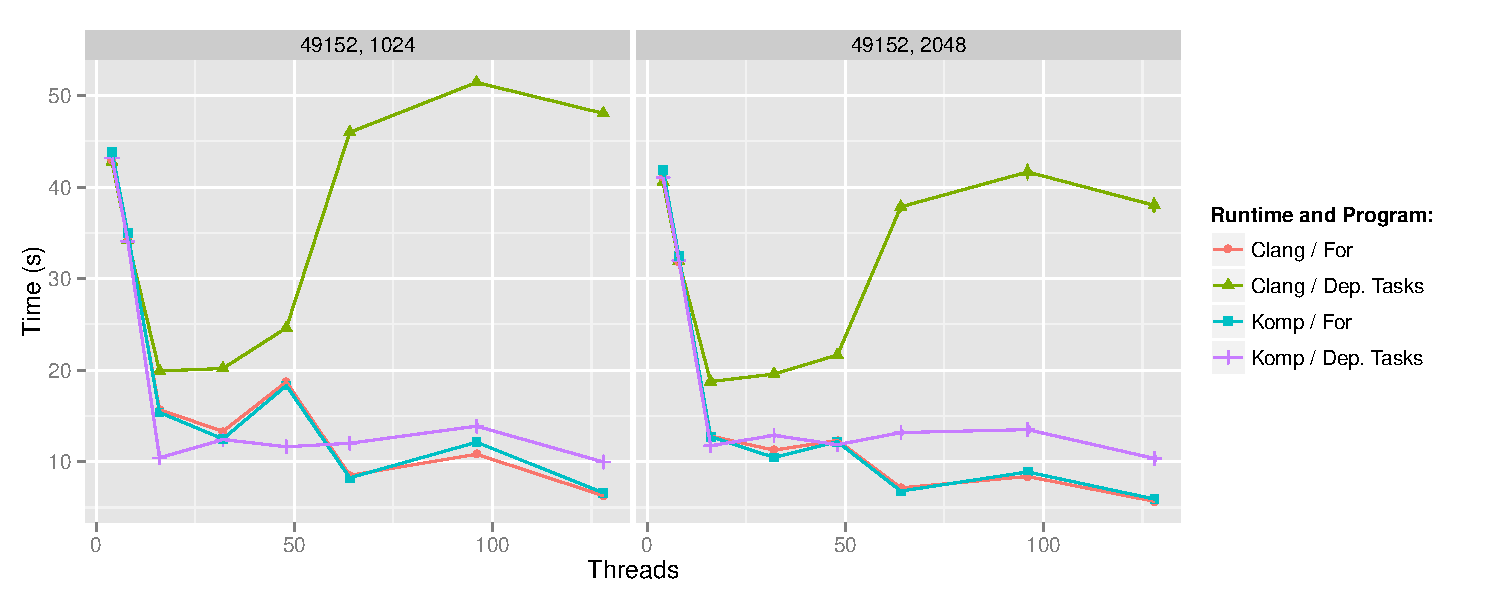
\includegraphics[width=\textwidth]{jacobi_scale_iomp_komp}
  \caption{Performances de Jacobi en fonction de la version et du support exécutif, avec une taille de matrice de 49152}\label{fig:contribs:perf_eval:eval-jacobi}
\end{figure}

La figure~\ref{fig:contribs:perf_eval:eval-jacobi} montre les performances de Jacobi sur deux tailles de blocs différentes.
Une distribution de données a été rajoutée dans l'application, avec également une affinité stricte suivant cette distribution de données sur les itérations successives.
Cela permet de garantir la réutilisation des données présentes dans le cache L2 (point critique pour cette application), et éviter des migrations de tâches inappropriées.
Les performances obtenues avec les versions à base de boucles sont faibles comparativement aux résultats de l'affinité, néanmoins cela vient du fait qu'il n'y a pas eu d'effort particulier de fait pour que le découpage des itérations correspondent à celui des distributions des données.
Les performances des deux versions devraient théoriquement être équivalentes~: l'affinité stricte est là pour restreindre la portée du vol de travail qui dégradait les performances, phénomène qui ne devrait pas être présent dans une version à base de boucles.



\subsection{Portage dans libOMP}\label{sec:contribs:perf_eval:libkomp}

Pendant le déroulement de cette thèse, les développeurs de Clang ont décidé d'adopter et d'intégrer officiellement le support exécutif d'Intel open source pour leur support d'OpenMP, et l'ont nommé libOMP.
Ce support exécutif dispose d'un support complet et robuste de la norme OpenMP~4.0, et utilise du vol de travail décentralisé (contrairement à libGOMP), avec également une découverte de la hiérarchie de la machine via hwloc.
Cela nous a donc semblé être une base favorable pour intégrer nos travaux et favoriser leur diffusion.
Les sections suivantes décrivent les modifications que nous avons effectués dans le support exécutif, et propose également une évaluation de performances pour valider leur implémentation.

\subsubsection{Extensions et options ajoutées}

Le support exécutif libOMP fonctionne, pour les tâches, par vol de travail.
Chaque threads dispose d'une file de tâches, et les stratégies d'ordonnancement sont les suivantes~: les tâches prêtes sont placées dans la file du thread courant~; lorsqu'un thread a besoin de voler du travail, il sélectionne aléatoirement une file de tâche d'un autre thread, s'il réussit un vol il reviendra voler cette victime la prochaine fois qu'il aura besoin de voler du travail.
D'après cette description, ce support exécutif dispose donc du minimum pour intégrer nos propositions.

Dans un premier temps, nous avons donc commencé par ajouter un ensemble de structures de données~: pour chaque nœud NUMA utilisés dans la \emph{team} OpenMP courante, nous avons ajouté une file de tâches, permettant ainsi d'exposer un second niveau de hiérarchie dans l'ordonnancement.
Nous avons également ajouté une file de tâche privée par thread et par nœud, afin de pouvoir implémenter facilement la notion d'affinité stricte.

Dans un second temps, nous avons modifié les fonctions de placement des tâches prêtes et de sélection d'une victime à voler.
Nous avons directement implémenté les stratégies présentées dans la section~\ref{sec:contrib:ws:heuristics} qui avaient le mieux fonctionné, à savoir~:
\begin{itemize}
  \item pour l'affinité entre une tâche et une donnée, le placement de la tâche est effectuée selon la stratégie \emph{pNumaWLoc}, définie dans la section~\ref{sec:openmp:runtime:push}.
  \item la sélection d'une file de tâche à voler se fait hiérarchiquement, dans l'ordre indiqué par la stratégie \emph{sNumaProc}, définis dans la section~\ref{sec:openmp:runtime:select}.
\end{itemize}

Dans la suite des expériences, nous appellerons ce support exécutif \emph{libKOMP}.

\subsubsection{Évaluation}

/!\ pour ces xp les versions de gcc/clang ont changé, ainsi que les BLAS !

\begin{figure}[ht]
  \centering
  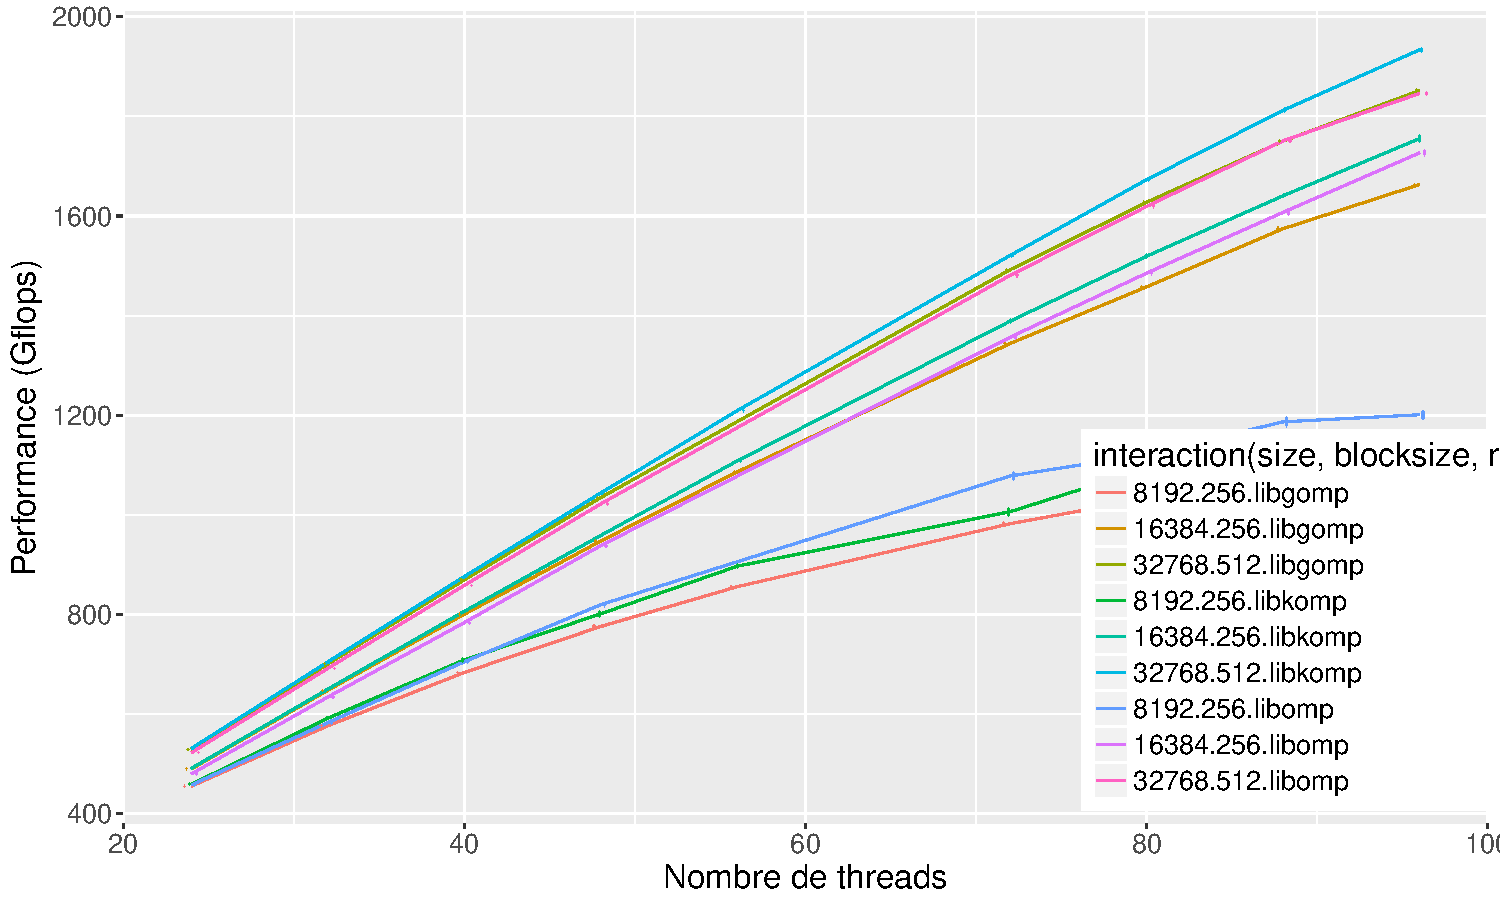
\includegraphics[width=\textwidth]{graph_all_cholesky_brunch}
  \caption{Graphe incomplet des perfs de cholesky sur brucnh}\label{fig:contribs:perf_eval:eval-cholesky-brunch}
\end{figure}

\begin{todo}
Finir les mesures pour le graphe (cf figure~\ref{fig:contribs:perf_eval:eval-cholesky-brunch}) et le commentaire.

C'est assez intéressant, parce qu'en fait l'affinité donne un clair avantage dès lors que les tailles de blocs font que la majorité des noyaux (gemm+trsm+syrk) sorte du cache !

Pour l'instant ma conclusion c'est qu'il faut commencer à regarder le dataset manipulé par les tâches pour prendre nos décisions (ce qui peut être évalué à travers le simulateur).
\end{todo}


\begin{todo}
  Il faut aussi comparer ça au simulateur. Peut être plus simplement faire une section à part.

  Vu que c'est principalement effectué avec le nouveau libkomp, peut être mettre ça dans une section suivant celle du "portage" vers le runtime intel.

  À discuter de où on met ça...
\end{todo}


